% Options for packages loaded elsewhere
% Options for packages loaded elsewhere
\PassOptionsToPackage{unicode}{hyperref}
\PassOptionsToPackage{hyphens}{url}
\PassOptionsToPackage{dvipsnames,svgnames,x11names}{xcolor}
%
\documentclass[
  12pt,
]{article}
\usepackage{xcolor}
\usepackage[margin=2.5cm]{geometry}
\usepackage{amsmath,amssymb}
\setcounter{secnumdepth}{5}
\usepackage{iftex}
\ifPDFTeX
  \usepackage[T1]{fontenc}
  \usepackage[utf8]{inputenc}
  \usepackage{textcomp} % provide euro and other symbols
\else % if luatex or xetex
  \usepackage{unicode-math} % this also loads fontspec
  \defaultfontfeatures{Scale=MatchLowercase}
  \defaultfontfeatures[\rmfamily]{Ligatures=TeX,Scale=1}
\fi
\usepackage{lmodern}
\ifPDFTeX\else
  % xetex/luatex font selection
\fi
% Use upquote if available, for straight quotes in verbatim environments
\IfFileExists{upquote.sty}{\usepackage{upquote}}{}
\IfFileExists{microtype.sty}{% use microtype if available
  \usepackage[]{microtype}
  \UseMicrotypeSet[protrusion]{basicmath} % disable protrusion for tt fonts
}{}
\makeatletter
\@ifundefined{KOMAClassName}{% if non-KOMA class
  \IfFileExists{parskip.sty}{%
    \usepackage{parskip}
  }{% else
    \setlength{\parindent}{0pt}
    \setlength{\parskip}{6pt plus 2pt minus 1pt}}
}{% if KOMA class
  \KOMAoptions{parskip=half}}
\makeatother
% Make \paragraph and \subparagraph free-standing
\makeatletter
\ifx\paragraph\undefined\else
  \let\oldparagraph\paragraph
  \renewcommand{\paragraph}{
    \@ifstar
      \xxxParagraphStar
      \xxxParagraphNoStar
  }
  \newcommand{\xxxParagraphStar}[1]{\oldparagraph*{#1}\mbox{}}
  \newcommand{\xxxParagraphNoStar}[1]{\oldparagraph{#1}\mbox{}}
\fi
\ifx\subparagraph\undefined\else
  \let\oldsubparagraph\subparagraph
  \renewcommand{\subparagraph}{
    \@ifstar
      \xxxSubParagraphStar
      \xxxSubParagraphNoStar
  }
  \newcommand{\xxxSubParagraphStar}[1]{\oldsubparagraph*{#1}\mbox{}}
  \newcommand{\xxxSubParagraphNoStar}[1]{\oldsubparagraph{#1}\mbox{}}
\fi
\makeatother


\usepackage{longtable,booktabs,array}
\usepackage{calc} % for calculating minipage widths
% Correct order of tables after \paragraph or \subparagraph
\usepackage{etoolbox}
\makeatletter
\patchcmd\longtable{\par}{\if@noskipsec\mbox{}\fi\par}{}{}
\makeatother
% Allow footnotes in longtable head/foot
\IfFileExists{footnotehyper.sty}{\usepackage{footnotehyper}}{\usepackage{footnote}}
\makesavenoteenv{longtable}
\usepackage{graphicx}
\makeatletter
\newsavebox\pandoc@box
\newcommand*\pandocbounded[1]{% scales image to fit in text height/width
  \sbox\pandoc@box{#1}%
  \Gscale@div\@tempa{\textheight}{\dimexpr\ht\pandoc@box+\dp\pandoc@box\relax}%
  \Gscale@div\@tempb{\linewidth}{\wd\pandoc@box}%
  \ifdim\@tempb\p@<\@tempa\p@\let\@tempa\@tempb\fi% select the smaller of both
  \ifdim\@tempa\p@<\p@\scalebox{\@tempa}{\usebox\pandoc@box}%
  \else\usebox{\pandoc@box}%
  \fi%
}
% Set default figure placement to htbp
\def\fps@figure{htbp}
\makeatother


% definitions for citeproc citations
\NewDocumentCommand\citeproctext{}{}
\NewDocumentCommand\citeproc{mm}{%
  \begingroup\def\citeproctext{#2}\cite{#1}\endgroup}
\makeatletter
 % allow citations to break across lines
 \let\@cite@ofmt\@firstofone
 % avoid brackets around text for \cite:
 \def\@biblabel#1{}
 \def\@cite#1#2{{#1\if@tempswa , #2\fi}}
\makeatother
\newlength{\cslhangindent}
\setlength{\cslhangindent}{1.5em}
\newlength{\csllabelwidth}
\setlength{\csllabelwidth}{3em}
\newenvironment{CSLReferences}[2] % #1 hanging-indent, #2 entry-spacing
 {\begin{list}{}{%
  \setlength{\itemindent}{0pt}
  \setlength{\leftmargin}{0pt}
  \setlength{\parsep}{0pt}
  % turn on hanging indent if param 1 is 1
  \ifodd #1
   \setlength{\leftmargin}{\cslhangindent}
   \setlength{\itemindent}{-1\cslhangindent}
  \fi
  % set entry spacing
  \setlength{\itemsep}{#2\baselineskip}}}
 {\end{list}}
\usepackage{calc}
\newcommand{\CSLBlock}[1]{\hfill\break\parbox[t]{\linewidth}{\strut\ignorespaces#1\strut}}
\newcommand{\CSLLeftMargin}[1]{\parbox[t]{\csllabelwidth}{\strut#1\strut}}
\newcommand{\CSLRightInline}[1]{\parbox[t]{\linewidth - \csllabelwidth}{\strut#1\strut}}
\newcommand{\CSLIndent}[1]{\hspace{\cslhangindent}#1}



\setlength{\emergencystretch}{3em} % prevent overfull lines

\providecommand{\tightlist}{%
  \setlength{\itemsep}{0pt}\setlength{\parskip}{0pt}}



 


\usepackage{booktabs}
\usepackage{longtable}
\usepackage{array}
\usepackage{multirow}
\usepackage{wrapfig}
\usepackage{float}
\usepackage{colortbl}
\usepackage{pdflscape}
\usepackage{tabu}
\usepackage{threeparttable}
\usepackage{threeparttablex}
\usepackage[normalem]{ulem}
\usepackage{makecell}
\usepackage{xcolor}
\makeatletter
\@ifpackageloaded{caption}{}{\usepackage{caption}}
\AtBeginDocument{%
\ifdefined\contentsname
  \renewcommand*\contentsname{Table of contents}
\else
  \newcommand\contentsname{Table of contents}
\fi
\ifdefined\listfigurename
  \renewcommand*\listfigurename{List of Figures}
\else
  \newcommand\listfigurename{List of Figures}
\fi
\ifdefined\listtablename
  \renewcommand*\listtablename{List of Tables}
\else
  \newcommand\listtablename{List of Tables}
\fi
\ifdefined\figurename
  \renewcommand*\figurename{Figure}
\else
  \newcommand\figurename{Figure}
\fi
\ifdefined\tablename
  \renewcommand*\tablename{Table}
\else
  \newcommand\tablename{Table}
\fi
}
\@ifpackageloaded{float}{}{\usepackage{float}}
\floatstyle{ruled}
\@ifundefined{c@chapter}{\newfloat{codelisting}{h}{lop}}{\newfloat{codelisting}{h}{lop}[chapter]}
\floatname{codelisting}{Listing}
\newcommand*\listoflistings{\listof{codelisting}{List of Listings}}
\makeatother
\makeatletter
\makeatother
\makeatletter
\@ifpackageloaded{caption}{}{\usepackage{caption}}
\@ifpackageloaded{subcaption}{}{\usepackage{subcaption}}
\makeatother
\usepackage{bookmark}
\IfFileExists{xurl.sty}{\usepackage{xurl}}{} % add URL line breaks if available
\urlstyle{same}
\hypersetup{
  pdftitle={Pulling the Wrong Lever: School Attainment, Open Data Analytics and Local Education Policy in England},
  pdfauthor={Adam Dennett; Natasha Priest; Tom Harrison; Dan Campbell-Meiklejohn},
  pdfkeywords={school attainment, education policy, school
absence, disadvantage gap, multilevel modelling, open data},
  colorlinks=true,
  linkcolor={blue},
  filecolor={Maroon},
  citecolor={Blue},
  urlcolor={Blue},
  pdfcreator={LaTeX via pandoc}}


\title{Pulling the Wrong Lever: School Attainment, Open Data Analytics
and Local Education Policy in England}
\usepackage{etoolbox}
\makeatletter
\providecommand{\subtitle}[1]{% add subtitle to \maketitle
  \apptocmd{\@title}{\par {\large #1 \par}}{}{}
}
\makeatother
\subtitle{Lessons from Brighton and Hove}
\author{Adam Dennett \and Natasha Priest \and Tom Harrison \and Dan
Campbell-Meiklejohn}
\date{2026-04-05}
\begin{document}
\maketitle
\begin{abstract}
The UK Government's 2026 schools white paper sets ambitious targets
including halving the disadvantage attainment gap and improving
attendance. Achieving these requires local education authorities to
understand the specific drivers of attainment in their areas. Using
multilevel linear mixed effects models fitted to all state-funded
secondary schools in England over four years (2021--22 to 2024--25), we
show that school-level Attainment 8 is highly predictable from a small
number of readily available variables. School-level absence is the most
powerful predictor, with a coefficient roughly 2.6 times larger than
concentrations of disadvantage. We apply these models to a case study of
Brighton and Hove, where admissions policy proposals in 2024 were
designed around the premise that attainment was `driven by economic
advantage'. Our analysis reveals that the city ranks among the
highest-performing local authorities once structural factors are
accounted for, but has the second worst absence rate in England. The
policy as designed was pulling a lever with relatively little mechanical
advantage while ignoring one with considerably more. We argue that the
Department for Education's open data provides the raw materials for
better local policy making, but a crucial gap exists between available
data and accessible, contextualised intelligence.
\end{abstract}


\section{Introduction}\label{introduction}

The outcomes of pupils attending schools are of perennial interest to
policy makers, given the established links to life outcomes (Farquharson
et al. 2024) and national economic productivity (Grant 2017). The UK
Government's 2026 schools white paper (DfE 2026) sets ambitious targets
including halving the disadvantage attainment gap, improving attendance,
reforming admissions and tackling place-based disadvantage. These
ambitions will require local education authorities (LEAs) to understand
the specific drivers of attainment in their areas and choose
interventions accordingly.

This paper argues that the Department for Education's (DfE) open data
provides most of the raw materials needed for such understanding, but a
crucial gap exists between data availability and accessible,
contextualised intelligence for decision makers. We demonstrate this
through an analysis of school-level attainment across England, combined
with a case study of Brighton and Hove where secondary school admissions
policy proposals in 2024--25 were designed around an incomplete
understanding of local attainment drivers.

Brighton and Hove provides a particularly instructive case. The city has
a distinctive admissions landscape featuring catchment areas with a
lottery tie-break for oversubscribed schools, introduced following
school closures in 2005 (Allen et al. 2013). In 2024, the council
launched proposals to reduce Published Admission Numbers at popular
schools and reserve places for out-of-catchment children, premised on
the belief that attainment was `driven by economic advantage' and that
redistributing disadvantaged pupils would narrow the attainment gap. The
response was overwhelmingly negative, yet the core policy direction
persisted through statutory consultation.

The authors are residents of Brighton and Hove with direct experience of
the effects of these proposals on their families and community. Some are
academics, some experienced in policy making, some involved in school
governance, and some simply parents. This diverse positionality
motivates the analysis: we argue that better analytical tools, applied
to readily available open data, could have substantially improved the
quality of the policy debate.

We are not claiming that this model is the best possible or that our
variable selection is optimal. Our intention is to show that with open,
freely available data and variables that are along the right lines, it
is possible to build a model explaining over 80\% of the variation in
school-level attainment with just a handful of predictors. When we know
the vast majority of influences on attainment and how they interact in
different local contexts, we can answer questions such as: `is changing
the social mix in schools likely to improve disadvantaged attainment?',
`what is the most important factor affecting attainment in a particular
LEA?', and `which schools are doing better or worse than expected?'.
Crucially, the effects can be presented not in standard deviations but
in policy-relevant GCSE points.

The paper proceeds as follows. We review the literature on secondary
school attainment drivers, then outline our modelling approach using DfE
open data. We present results showing which factors matter most and how
they interact, before applying these findings to Brighton and Hove. We
conclude with implications for local and national education policy.

\section{Literature review}\label{literature-review}

\subsection{Socio-economic background and
disadvantage}\label{socio-economic-background-and-disadvantage}

The Education Policy Institute's annual reports document that by the
time pupils sit their GCSEs, disadvantaged pupils are on average around
18 months of learning behind their more affluent peers, a gap that
narrowed modestly after 2011 but partially reversed following the
COVID-19 pandemic (Tuckett et al. 2023). Free School Meal (FSM)
eligibility serves as the standard proxy for disadvantage, though its
limitations are well established. Stopforth and Gayle (2025) demonstrate
that finer-grained measures of parental social class reveal persistent
attainment gaps that FSM-based analyses tend to understate.

A crucial dimension is that inequalities at GCSE level are substantially
mediated by prior attainment at Key Stage 2 (KS2). Gorard and Siddiqui
(2019) show that the duration of disadvantage is a stronger predictor
than disadvantage at any single point. They also propose that pupils do
worse in schools with concentrations of disadvantage, estimating
improvements of 0.05--0.15 standard deviations from greater social
mixing --- approximately one GCSE grade in one subject. However, the
claim that mixing can be achieved at `almost no cost' is a conjecture
that overlooks the real-world consequences for communities.

\subsection{Attendance}\label{attendance}

School attendance is among the strongest predictors of attainment. DfE
analysis of 2018/19 data (DfE 2022) documents a stark gradient: among
persistently absent pupils, only 35.6\% achieved a standard pass in
English and Maths, compared with 83.7\% among those with no recorded
absences. More recent analysis finds that pupils with near-perfect
attendance were 1.9 times as likely to achieve a grade 5 pass compared
with otherwise similar pupils attending 90--95\% of the time (DfE
2025a). Dräger et al. (2024), using the 1970 British Cohort Study, find
that absences at age 10 are associated with lower educational attainment
in adulthood. The Social Mobility Commission (Riordan et al. 2021)
conclude that the correlation between attendance and progress is `most
likely to be causal'.

Post-pandemic persistent absence has risen sharply, from around 10.5\%
pre-pandemic to approximately 21.9\% in secondary schools by 2023/24,
with rates for FSM-eligible pupils around 32\% (DfE 2025b). This
compounds the challenge of disentangling school-level from pupil-level
effects.

\subsection{Other factors}\label{other-factors}

Prior attainment at KS2 reflects accumulated inequalities from before
secondary school (Gorard and Siddiqui 2019; Stopforth and Gayle 2025).
Ethnic inequalities are persistent (Gillborn et al. 2017), though Gorard
et al. (2025) show these are substantially reduced when controlling for
pupil-level characteristics. The underperformance of disadvantaged White
British pupils, particularly boys, has attracted policy attention, with
causes contested between place-based deprivation and cultural factors
(Strand 2021; Commons Education Committee 2021).

School-level selectivity inflates raw performance metrics. Anders et al.
(2024) find that the private school premium effectively disappears once
socioeconomic background is controlled for. Simon Burgess et al. (2018)
show grammar schools reinforce socio-economic stratification without
overall attainment benefits.

Workforce factors including effective leadership (Zuccollo et al. 2023),
teaching quality (Simon Burgess et al. 2023; S. Burgess et al. 2022),
and teacher retention (Gibbons et al. 2018; Menzies 2023) contribute to
variation in attainment, with effects felt most acutely by disadvantaged
students (Allen et al. 2018). The `London Effect' (Ross et al. 2020)
reflects a localised concentration of agency factors --- parental
expectations, homework hours, lower unauthorised absence --- rather than
a purely geographic phenomenon.

The factors affecting attainment are multifaceted and interrelated.
Synthesising their relative contributions requires an analysis combining
them simultaneously, which is where we now turn.

\section{Data and methods}\label{data-and-methods}

\subsection{Data}\label{data}

The DfE publishes extensive open data on schools via its statistical
services. We assembled a panel dataset covering the four post-COVID
academic years (2021--22 to 2024--25), linking school performance,
absence, pupil population, workforce and Ofsted data. Data
pre-processing details are available in the supplementary
material.\footnote{Supplementary material:
  \url{https://adamdennett.github.io/school_attainment_tool/}} The final
analysis panel comprises 13,419 school-year observations from 3,523
academies and maintained schools across 152 LEAs. Independent schools,
colleges and special schools are excluded. All data are school-level
aggregates; interpretations relate to this level of aggregation.

\subsection{Model specification}\label{model-specification}

We fit multilevel linear mixed effects models (LMEs) with schools nested
within LEAs within regions (Snijders 2012). The outcome is
log-transformed Attainment 8, the measure cited in the DfE (2026) white
paper. Because the outcome is on the log scale, coefficients for
log-transformed predictors represent elasticities.

The model specification is:

\[
\log(\text{ATT8}_{ij}) = \beta_0 + \sum_{k=1}^{9} \beta_k \, x_{kij} + u_{\text{year}} + u_{\text{Ofsted}} + u_{\text{region}} + u_{\text{LA|region}} + \varepsilon_{ij}
\]

where \(i\) indexes schools, \(j\) indexes year-observations, the
\(\beta_k\) are fixed-effect coefficients, and the \(u\) terms are
random-effect intercepts for year, Ofsted rating, region, and LEA nested
within region.

Fixed-effect predictors comprise: log(\% FSM-eligible), log(\% overall
absence), log(\% EAL), \% low prior attainment at KS2, selective
admissions (dummy), Gorard Segregation Index (LA-level), teacher
retention rate, leadership pay proportion, and log(teacher sickness
days). Variable selection was informed by the literature review and by
the policy narrative in Brighton and Hove, where segregation featured
prominently.

We fit separate models for overall Attainment 8, disadvantaged-pupil
Attainment 8, and non-disadvantaged-pupil Attainment 8, as both panel
models (all four years) and individual year models. Models were
estimated using the \texttt{lme4} package in R with REML estimation.

\section{Results}\label{results}

\subsection{Model fit}\label{model-fit}

The models explain a substantial proportion of variance in school-level
Attainment 8. For all pupils, the conditional \(R^2\) (fixed plus random
effects) is 0.77, with marginal \(R^2\) (fixed effects alone) of 0.63.
For disadvantaged pupils the conditional \(R^2\) is 0.73; for
non-disadvantaged pupils, 0.79. School-level attainment is remarkably
predictable from these structural factors.

\subsection{Stepwise decomposition}\label{stepwise-decomposition}

\begin{table}

\caption{\label{tbl-stepwise}Stepwise progression to the full multilevel
model for overall Attainment 8.}

\centering{

\centering\begingroup\fontsize{7}{9}\selectfont

\resizebox{\ifdim\width>\linewidth\linewidth\else\width\fi}{!}{
\begin{tabular}[t]{lrlrlrlrlrl}
\toprule
\multicolumn{1}{c}{ } & \multicolumn{2}{c}{M1: FSM} & \multicolumn{2}{c}{M2: +Absence} & \multicolumn{2}{c}{M3: +Prior} & \multicolumn{2}{c}{M4: All fixed} & \multicolumn{2}{c}{M5: Full LME} \\
\cmidrule(l{3pt}r{3pt}){2-3} \cmidrule(l{3pt}r{3pt}){4-5} \cmidrule(l{3pt}r{3pt}){6-7} \cmidrule(l{3pt}r{3pt}){8-9} \cmidrule(l{3pt}r{3pt}){10-11}
Variable & Est. & t & Est.  & t  & Est.   & t   & Est.    & t    & Est.     & t    \\
\midrule
(Intercept) & 4.473*** & 621.25 & 5.006*** & 579.97 & 4.833*** & 547.18 & 4.628*** & 319.11 & 4.633*** & 125.61\\
log(% FSM) & -0.201*** & -88.94 & -0.122*** & -59.66 & -0.073*** & -33.46 & -0.071*** & -28.60 & -0.067*** & -24.90\\
log(% Absence) &  &  & -0.364*** & -82.87 & -0.287*** & -65.28 & -0.242*** & -51.65 & -0.213*** & -46.03\\
log(% EAL) &  &  &  &  &  &  & 0.014*** & 13.69 & 0.006*** & 4.92\\
% Low Prior Attainment &  &  &  &  & -0.006*** & -45.75 & -0.005*** & -37.59 & -0.006*** & -41.35\\
Admissions: Other non-selective &  &  &  &  &  &  & 0.051*** & 11.01 & 0.001 & 0.08\\
Admissions: Selective &  &  &  &  &  &  & 0.140*** & 19.96 & 0.108*** & 16.20\\
Gorard Segregation &  &  &  &  &  &  & 0.052 & 1.92 & -0.033 & -0.69\\
Teacher Retention &  &  &  &  &  &  & 0.001*** & 12.92 & 0.000*** & 10.20\\
Leadership Pay % &  &  &  &  &  &  & -0.001*** & -6.10 & -0.001*** & -5.39\\
log(Teacher Sickness) &  &  &  &  &  &  & -0.016*** & -6.08 & -0.015*** & -6.17\\
Random effects &  &  &  &  &  &  &  &  &  & \\
Year &  &  &  &  &  &  &  &  & 0.030 & (SD)\\
Ofsted rating &  &  &  &  &  &  &  &  & 0.017 & (SD)\\
Region &  &  &  &  &  &  &  &  & 0.047 & (SD)\\
LA (nested in region) &  &  &  &  &  &  &  &  & 0.044 & (SD)\\
Residual &  &  &  &  &  &  &  &  & 0.094 & (SD)\\
 &  &  &  &  &  &  &  &  &  & \\
R² & 0.393 &  & 0.612 &  & 0.669 &  & 0.693 &  & 0.632 & (marginal)\\
R² (conditional) &  &  &  &  &  &  &  &  & 0.771 & (fixed + random)\\
N & 12,210 &  & 12,210 &  & 12,210 &  & 12,210 &  & 12,210 & \\
\bottomrule
\end{tabular}}
\endgroup{}

}

\end{table}%

The stepwise progression in Table~\ref{tbl-stepwise} reveals the
mediating structure among the key predictors. In Model 1, the FSM
coefficient is --0.201. Adding absence in Model 2 halves it to --0.122,
as absence absorbs much of the explanatory power previously attributed
to deprivation. Adding prior attainment in Model 3 reduces both FSM and
absence coefficients further. By Model 3, with just three variables,
approximately two-thirds of attainment variation is explained.

Model 4 adds additional fixed effects including EAL proportions,
selective admissions, workforce variables and the Gorard Segregation
Index. Model 5 adds random effects for year, Ofsted rating, region and
LEA nested within region, lifting the conditional \(R^2\) from 0.63
(marginal) to approximately 0.77, indicating that 14\% of attainment
variance is tied to these grouping factors --- capturing unmeasured
factors such as school culture, leadership quality, local authority
support services, and community characteristics.

The Gorard Segregation Index is not statistically significant in Models
4 or 5. Once a school's own FSM levels, attendance, prior attainment and
geographic location are accounted for, the distribution of disadvantaged
students across schools within an LEA adds no predictive power. Any harm
that segregation causes is fully mediated by the variables already in
the model. We include it because segregation arguments formed much of
the justification for the Brighton and Hove admissions proposals.

A crucial feature of these models is that the log-transformed variables
encode non-linear relationships. The same percentage-point change
produces different effects depending on where a school starts. For
concentrations of disadvantage, the relationship between FSM and
attainment flattens above about 20\% FSM --- further increases in
disadvantage do not correlate with noticeable further declines. Most of
the strong effect appears below 15\%, where further reductions are
correlated with much steeper attainment increases. This non-linearity
has direct policy consequences: individual LEAs need to consider
carefully where each school sits on the distribution to appreciate what
changes might realistically achieve.

\subsection{Relative variable
importance}\label{relative-variable-importance}

\begin{figure}

\centering{

\pandocbounded{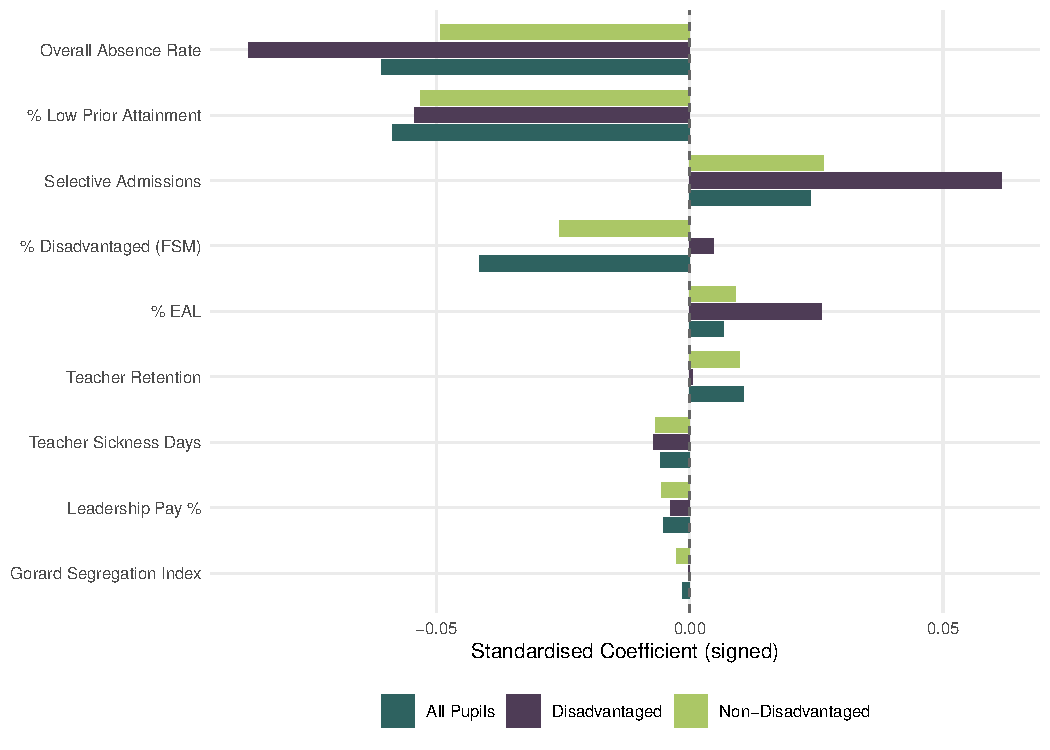
\includegraphics[keepaspectratio]{JEP_Paper_files/figure-pdf/fig-standardised-coefficients-1.pdf}}

}

\caption{\label{fig-standardised-coefficients}Standardised coefficients
showing relative variable importance across pupil groups. Bars show the
change in log(ATT8) associated with a one-SD shift in each predictor.}

\end{figure}%

Figure~\ref{fig-standardised-coefficients} compares the standardised
coefficients across all three pupil groups. Absence is the dominant
predictor across all groups, and even more important for disadvantaged
pupils --- nearly half of the variation in school-level performance for
this group is explained by attendance alone.

The most contentious finding concerns concentrations of disadvantage.
For non-disadvantaged pupils, higher FSM proportions are associated with
lower attainment. But for disadvantaged pupils, the coefficient is
\emph{positive} --- after controlling for absence and prior attainment,
disadvantaged pupils perform slightly better in schools with higher
concentrations of other disadvantaged pupils. This finding is robust
across individual year models and alternative specifications of
disadvantaged attainment and disadvantage measures.\footnote{See
  supplementary material for robustness checks:
  \url{https://adamdennett.github.io/school_attainment_tool/model_experiments.html}}
In the full multilevel model, this positive coefficient shrinks
substantially, suggesting the effect operates through LEA-level and
Ofsted-level factors rather than concentration per se --- schools with
higher FSM proportions in certain LEAs appear to have developed
effective support systems, possibly through targeted use of Pupil
Premium funding.

For non-disadvantaged pupils, the effects of higher disadvantage
concentrations are more clearly negative. Even after controlling for
attendance and prior scores, being in a higher-disadvantage school
depresses Attainment 8 for this group --- a possible peer effect or
curriculum-resourcing dynamic.

Absence remains consistently the biggest predictor across all groups and
is even more important for disadvantaged pupils. Nearly half of the
difference in school-level performance for disadvantaged pupils is
explained simply by whether they attend. Disadvantaged pupils lack the
safety net of engaged parents, private tutors or revision resources that
some less disadvantaged students have, making them more reliant on
classroom instruction. In this sense, attendance is the ultimate equity
lever.

We do not advocate for concentrating disadvantaged pupils. However,
deconcentration policies premised on the assumption that disadvantaged
pupils inevitably fare worse in higher-poverty schools are not supported
by this evidence. And where such policies require longer journeys that
risk increasing absence, they could be actively counterproductive.

\section{Brighton and Hove case
study}\label{brighton-and-hove-case-study}

\subsection{Local context}\label{local-context}

Brighton and Hove has ten secondary schools: six community schools run
by the LEA, two academies (Brighton Aldridge Community Academy --- BACA
--- and Portslade Aldridge Community Academy --- PACA) and two church
schools that set their own admissions. Following school closures in the
east of the city in 2005, large catchment areas were introduced with a
lottery tie-break for oversubscribed schools --- making admissions very
different to most other places in England where distance typically
determines priority (Allen et al. 2013).

Following the 2023 local elections, the Labour Party took overall
control and implemented a Leader and Cabinet system, concentrating
decision-making power. In October 2024, the council launched proposals
to reduce Published Admission Numbers at popular central schools, redraw
catchment boundaries, and reserve 20\% of places in some schools for
out-of-catchment children. The stated aims were to improve educational
outcomes for disadvantaged pupils and ensure financial viability of
under-subscribed peripheral schools. Underpinning the proposals was an
assertion that attainment in the city was `driven by economic advantage'
and that redistributing disadvantaged pupils would narrow the attainment
gap, drawing on the work of Gorard and Siddiqui (2019) on school
segregation.

The public response was overwhelmingly negative, with the council's own
feedback summary noting `a strong preference for improving existing
schools rather than redistributing students, alongside deep concerns
about potential impacts on community cohesion and student wellbeing'.
The proposals would, by the council's own calculations, force
significant numbers of children from central catchments to attend
schools at the periphery of the city, potentially requiring over two
hours of daily commuting.

From the papers accompanying the proposals and the content of the
scrutiny committee meetings, it was clear the council had settled on
affecting increased social mixing --- beyond levels already in the top
third nationally --- in the belief this would raise disadvantaged
attainment. This was in addition to a 2023 policy giving FSM-eligible
pupils priority in admissions, which was already affecting further
mixing without opposition. That the central catchments were perceived as
more `middle-class' and the peripheral schools, particularly in the east
of the city, as more `working-class', may have factored into this
design.

Whether the availability of better evidence would have changed the
political outcome is unknowable. But having been on the side of the city
responding to proposals rather than generating them, we can say that
accessible evidence \emph{would} have enabled earlier and more
constructive engagement. The compressed consultation timeline left
wholly inadequate time to assemble and present counter-evidence for the
complexity of the issues at stake. What follows is an attempt to
demonstrate what that evidence looks like.

\subsection{Local authority effects}\label{local-authority-effects}

\begin{figure}

\centering{

\pandocbounded{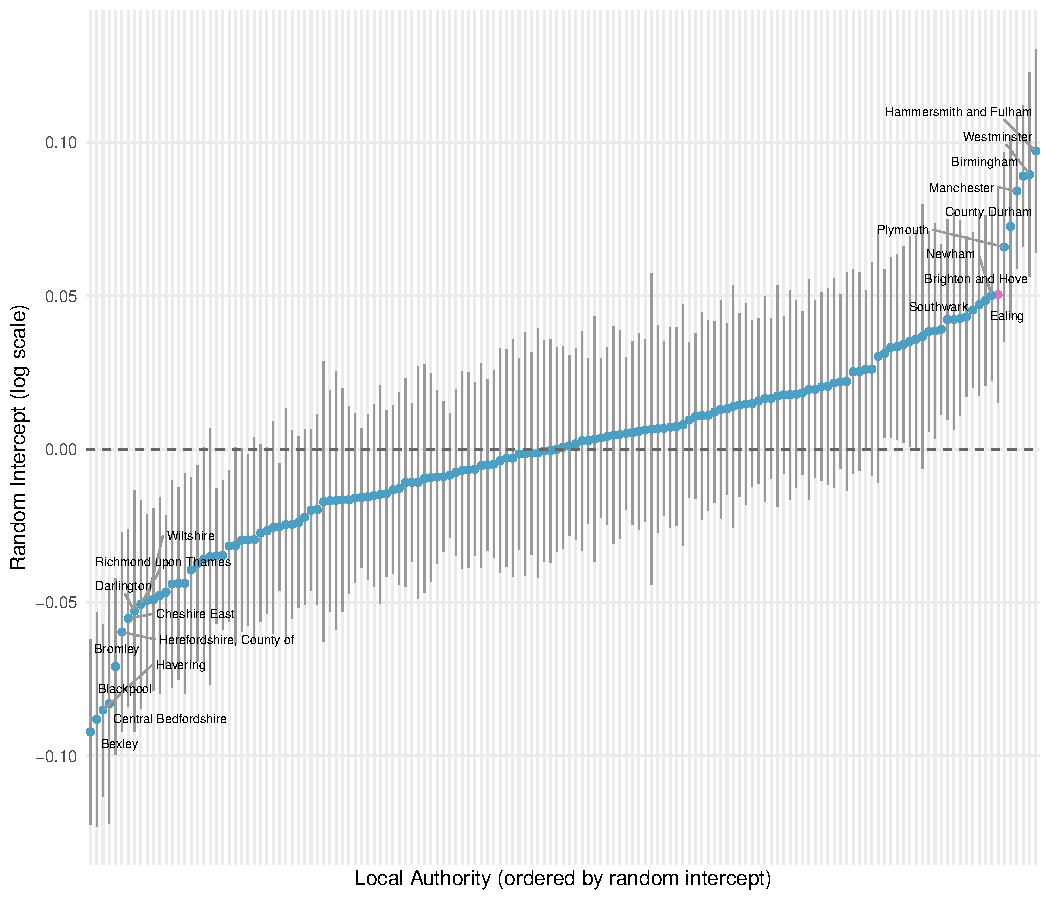
\includegraphics[keepaspectratio]{JEP_Paper_files/figure-pdf/fig-caterpillar-1.pdf}}

}

\caption{\label{fig-caterpillar}LA random intercepts for
disadvantaged-pupil attainment (imputed full panel model). Top and
bottom 10 LAs labelled; Brighton and Hove highlighted.}

\end{figure}%

Figure~\ref{fig-caterpillar} shows that Brighton and Hove ranks 7th out
of 152 LEAs for disadvantaged attainment once structural factors are
accounted for. For non-disadvantaged pupils it ranks 5th; for all
pupils, 4th. The positive random intercept of approximately +0.06
translates to around a 6\% uplift in Attainment 8 --- roughly 2 GCSE
points above what structural factors would predict. This was unknown at
the time of the 2024 consultation and entirely absent from the public
narrative, which was framed around a premise of failure.

\subsection{Comparing policy levers: absence versus
disadvantage}\label{comparing-policy-levers-absence-versus-disadvantage}

Because the model uses log-transformed variables, the same
percentage-point change produces different effects depending on where a
school starts --- returns \emph{accelerate} as values improve.
Figure~\ref{fig-accelerating-returns} places both the absence and FSM
levers on a common y-axis.

\begin{figure}

\centering{

\pandocbounded{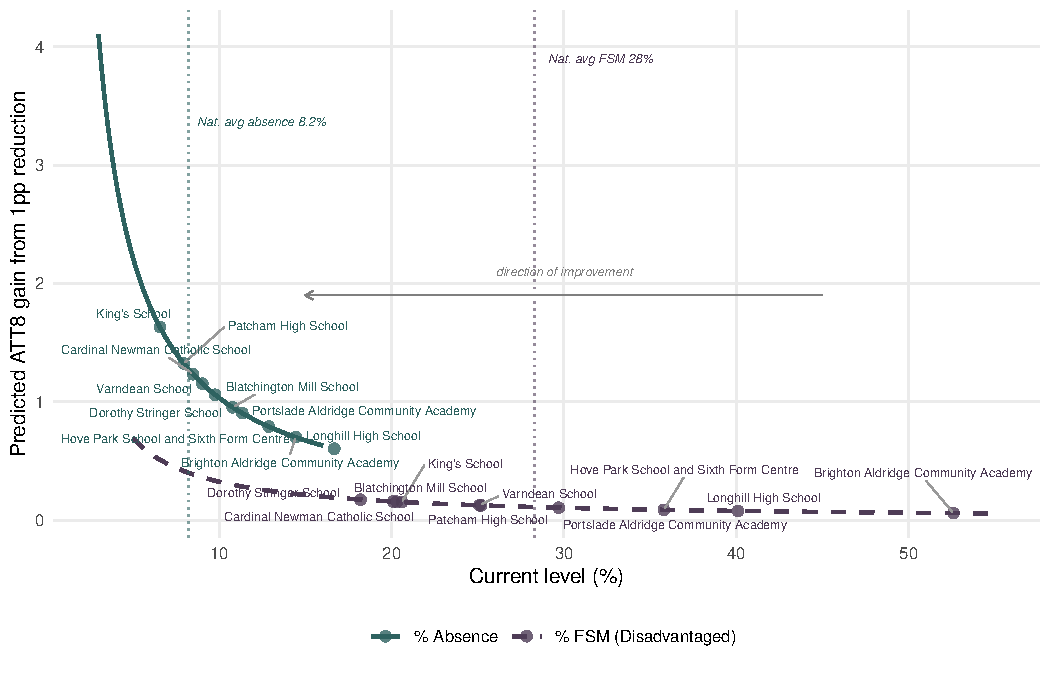
\includegraphics[keepaspectratio]{JEP_Paper_files/figure-pdf/fig-accelerating-returns-1.pdf}}

}

\caption{\label{fig-accelerating-returns}Accelerating returns: each
percentage-point reduction buys a progressively larger ATT8 gain
(reading right to left). Absence delivers substantially larger gains
than FSM at every level. Brighton and Hove schools marked on each
curve.}

\end{figure}%

Three features are immediately visible. First, the absence curve sits
above the FSM curve at every starting level. Second, the gap
\emph{widens} as values improve. Third, Brighton and Hove schools
cluster in the flatter right-hand portion for both variables, but the
city's position is far more extreme on absence.

Brighton and Hove's mean school FSM rate (28.8\%) is close to the
national average (28.3\%). But the city's mean absence rate (10.8\%)
against a national average of 8.2\% places it at the 99th percentile ---
among the very worst in England. When standardised by the city's spread,
the absence coefficient is 2.6 times as important as FSM for predicting
attainment.

Bringing schools above the national average for absence down to it would
produce predicted gains averaging +2.9 Attainment 8 points per school,
with gains for disadvantaged pupils averaging +3.3 points. Even dramatic
FSM reductions would yield gains closer to 1 point. The policy was
pulling a lever with relatively little mechanical advantage while
ignoring one with considerably more.

\subsection{Contextualised school
performance}\label{contextualised-school-performance}

\begin{figure}

\centering{

\pandocbounded{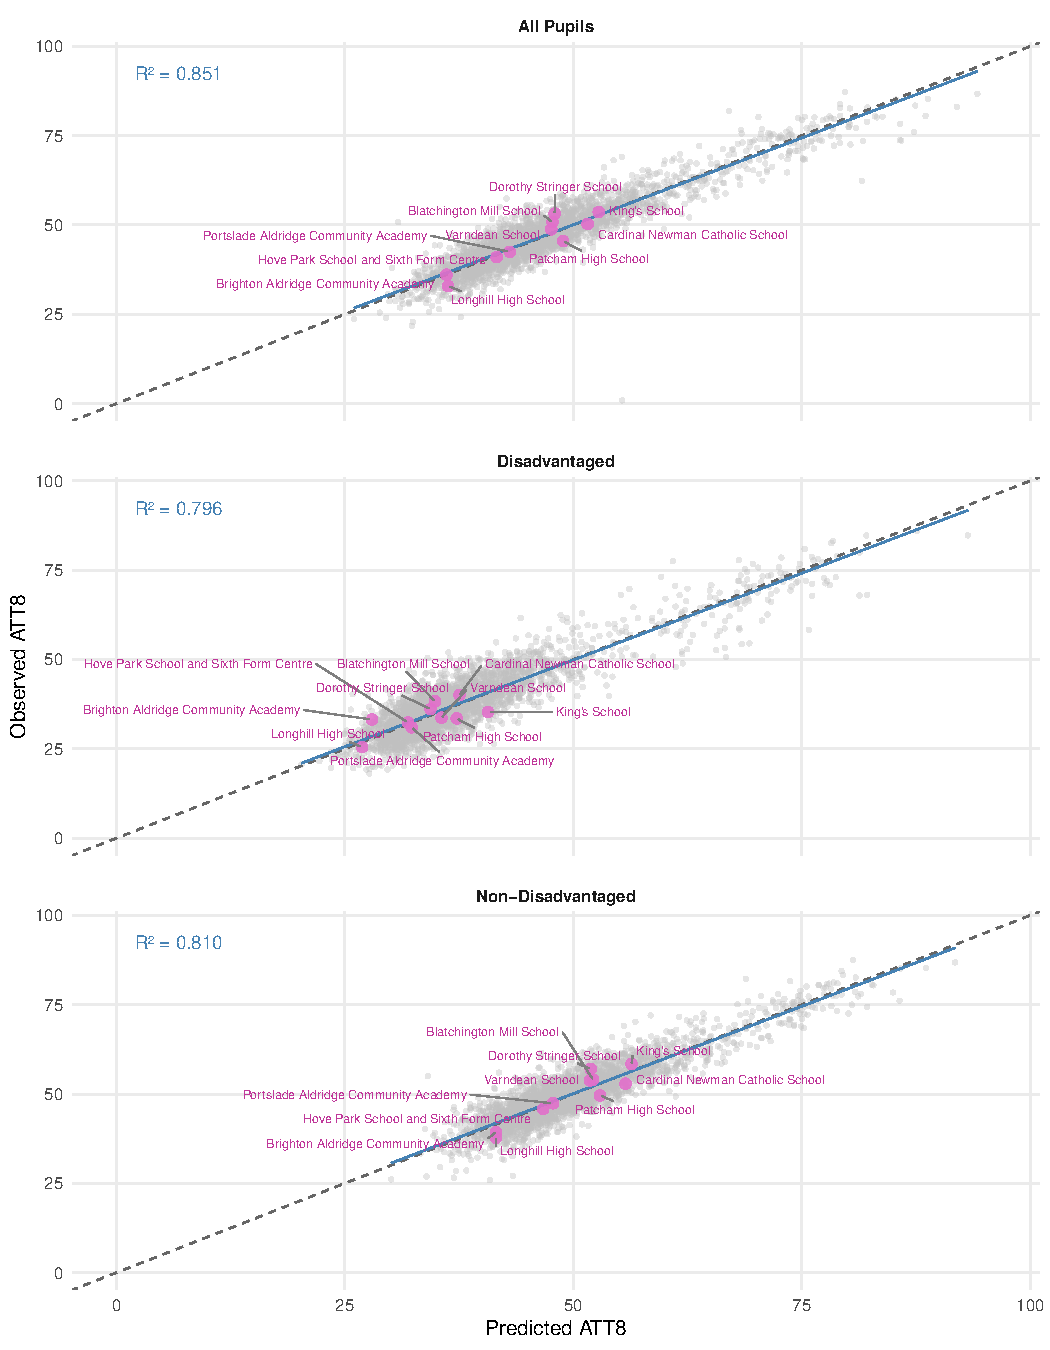
\includegraphics[keepaspectratio]{JEP_Paper_files/figure-pdf/fig-obs-vs-pred-1.pdf}}

}

\caption{\label{fig-obs-vs-pred}Observed versus predicted Attainment 8
for Brighton and Hove schools (highlighted) against all schools
nationally, 2024--25.}

\end{figure}%

Figure~\ref{fig-obs-vs-pred} shows observed versus predicted Attainment
8 for the latest year. The model residuals --- the vertical distance
from the diagonal --- provide contextualised `value-added' measures. Two
cases are particularly instructive. Brighton Aldridge Community Academy
(BACA), situated in one of the city's most deprived areas, is the
best-performing school for disadvantaged pupils once intake is accounted
for, with a residual of approximately +5 Attainment 8 points in
2024--25. During the consultation, BACA's `Requires Improvement' Ofsted
rating and low raw scores led a campaign group to encourage parents to
choose other schools. Many opted for Patcham High School, which in raw
terms appears mid-table but has consistently negative value-added
residuals for disadvantaged pupils. BACA's April 2025 Ofsted upgrade to
`Good' in all areas vindicated what the data already showed, but came
too late for families who had already made decisions based on incomplete
signals.

\section{Discussion}\label{discussion}

\subsection{The danger of single-lever policy
thinking}\label{the-danger-of-single-lever-policy-thinking}

The Brighton and Hove experience illustrates what happens when policy
makers latch onto a single causal narrative. The council's 2024
proposals were built almost entirely on the premise that redistributing
disadvantaged pupils would narrow the attainment gap. Our analysis
suggests this was at best an incomplete understanding and at worst a
policy with many losers and few clear winners. Concentrations of
disadvantage are one of the weaker available levers, and for
disadvantaged pupils specifically the direction of the effect runs
contrary to the policy assumptions. Reducing absence to the national
average at the worst-affected schools could yield gains of 3--5 GCSE
points; even dramatic FSM reductions would yield closer to 1--2 points.

Moreover, the chosen lever carried its own risks. Longer journeys
imposed by redistribution policies are associated with higher absence
(Thomson 2023) --- precisely the factor that most drags on attainment.
The claim that social mixing can be achieved at `almost no cost' (Gorard
and Siddiqui 2019) overlooks these second-order effects.

\subsection{Absence as the primary policy
lever}\label{absence-as-the-primary-policy-lever}

Perhaps the most striking finding is the complete absence of absence
from the policy narrative. The city had the second worst absence rate in
England in 2024--25 and has been consistently among the worst in
England. Yet absence was not part of the policy conversation. The irony
is considerable: the city ranks best 7th for disadvantaged attainment
after structural adjustments, but this strong underlying performance is
being dragged down by an extreme absence problem.

Brighton and Hove's absence rates are not a necessary consequence of its
intake composition. The city has near-average FSM levels but near-worst
absence, suggesting the problem is driven by local factors ---
attendance culture, enforcement practices, or community dynamics ---
rather than being an unavoidable correlate of disadvantage.

\subsection{The BACA paradox and contextualised
benchmarking}\label{the-baca-paradox-and-contextualised-benchmarking}

The case of BACA offers a particularly sharp illustration of the damage
done when school quality is assessed through crude metrics. During and
after the 2024 consultation, a vocal campaign emerged from the BACA
catchment demanding that parents have more `choice' of schools and
implicitly through this narrative encouraging parents to seek
alternatives. Data released as part of objections to the Schools
Adjudicator revealed that many families opted for Patcham High School
--- rated `Good' by Ofsted and sitting comfortably mid-table in raw
league tables. But at the time, all most parents would have known about
BACA was its `Requires Improvement' Ofsted rating and low raw attainment
figures.

The contextualised analysis tells a very different story. BACA, situated
in one of the city's most deprived areas with around 50\% FSM-eligible
pupils and 30\% low prior attainment, is the best-performing school in
the city for disadvantaged pupils once structural factors are controlled
for. A disadvantaged pupil at BACA in 2024--25 left with GCSEs around 5
points higher than comparable pupils at similar schools elsewhere in
England; the four-year average was around 3 points --- a boost far
exceeding any fraction-of-a-point differences achievable through
altering the disadvantage mix, even before accounting for likely
increased absence from longer journeys. BACA in many ways exemplifies
the national finding that disadvantaged pupils perform better in schools
with higher concentrations of disadvantage, likely because such schools
develop specialised support systems through targeted use of Pupil
Premium and other resources.

By contrast, Patcham --- the school many BACA-catchment parents chose
--- has consistently negative value-added residuals for disadvantaged
pupils, with a four-year average around --2.6 points. These differences
have been hidden by the school's comfortable mid-table raw attainment
position, which largely reflects its more advantaged intake rather than
educational effectiveness. Parents, acting rationally on the basis of
available information, were choosing the objectively worse option for
their children's GCSE outcomes. This is not a criticism of those parents
--- they were operating in a knowledge vacuum. It is, however, a
powerful argument for the kind of contextualised benchmarking made
public this analysis makes possible.

\subsection{Conflicting incentives: viability versus
attainment}\label{conflicting-incentives-viability-versus-attainment}

It is worth acknowledging what was only partially articulated during the
consultation: that a significant driver of the proposals was financial
rather than educational. Reducing PANs at popular schools and creating
out-of-catchment priority places were designed, at least in part, to
redirect pupil flows toward under-subscribed peripheral schools. Keeping
such schools financially viable is a legitimate concern. However, there
is an inherent tension between optimising for financial sustainability
and optimising for educational outcomes. If the net effect is to move
children from schools adding more value to schools adding less, the
aggregate impact on city-wide attainment could be negative. The
financial and educational cases needed to be weighed transparently, and
it is not clear this trade-off was adequately acknowledged.

Following widespread opposition and appeals to the Schools Adjudicator,
the proposed PAN reductions were rejected and the 20\% out-of-catchment
priority was reduced to 5\%. While displacement was minimised, the
policy reverberations continued through the choices expressed by parents
already influenced by the preceding debate.

\subsection{The cost of speed over
evidence}\label{the-cost-of-speed-over-evidence}

The institutional context deserves reflection. The shift to a Leader and
Cabinet system concentrated decision-making power and enabled policy to
be enacted through a whipped voting system. The consultation was
compressed in timeline and limited in scope for deliberative engagement.
This matters because the evidence base for school attainment is complex
--- the factors are multiple, interacting, non-linear and
context-dependent. Institutional structures that compress deliberation
timelines are particularly dangerous when the evidence requires careful
handling and its implications are counterintuitive. Had the analysis
presented here been available at the outset, the quality of public
scrutiny would have been substantially higher, even if the political
outcome had remained the same.

\subsection{Implications for national
policy}\label{implications-for-national-policy}

The DfE (2026) white paper's ambitions will founder if pursued at the
local level without adequate analytical infrastructure. Every LEA
occupies different positions along the non-linear curves that relate
predictors to outcomes. What works in one context may be
counterproductive in another. The DfE's open data provides most of the
raw materials, but there is a crucial gap between raw data availability
and the accessible, contextualised intelligence that decision makers
need.

We have developed an interactive Policy Simulator tool,\footnote{School
  Attainment Policy Simulator:
  \url{https://adam-dennett.shinyapps.io/School_Attainment_Policy_Simulator/}}
underpinned by the models in this paper, to begin bridging that gap. The
tool allows users to explore any school in England, compare against
contextual expectations, and model the indicative impact of changes to
key variables.

\subsection{Limitations}\label{limitations}

These are school-level models built from aggregate published data, not
pupil-level analyses. The associations identified are not experimental
causal estimates but the best approximations available from
observational data. The models cannot capture unmeasured factors such as
school culture, parental engagement, or individual pupil resilience. The
Policy Simulator translates associations into indicative, not
definitive, projections. We do not claim that reducing absence by a
given amount will mechanically produce the predicted gain --- the real
world is more complex than any model captures. What we do claim is that
these models are accurate enough, and the patterns consistent enough
across years and specifications, to substantially improve the quality of
the conversation around what matters most.

\section{Conclusion}\label{conclusion}

This paper has demonstrated that the DfE's open data is a substantially
underutilised resource for understanding school attainment. School-level
Attainment 8 is remarkably predictable from a small number of variables,
and that predictability creates opportunities for better-informed local
policy. The Brighton and Hove case study --- motivated by the authors'
direct experience of a flawed consultation process --- provides a
cautionary illustration of what happens when policy is anchored to a
single causal narrative without adequate regard for the full evidence
base.

Our recommendations are directed at three audiences. For the DfE: invest
in analytical infrastructure at the local level and consider how
contextualised benchmarking tools might be developed at scale. For LEAs:
resist single causal narratives and create institutional space for
genuine deliberation before irreversible decisions. The factors
affecting attainment are multiple, interacting, non-linear and
context-dependent. For schools, governors and parents: contextualised
benchmarking offers a fairer basis for understanding school quality than
raw scores or single-word Ofsted ratings.

The challenge is to ensure that this understanding reaches decision
makers in a usable form \emph{before} decisions are made --- not after.
The raw materials already exist. What is needed is the analytical
capacity and institutional willingness to use them.

\section*{Acknowledgements}\label{acknowledgements}
\addcontentsline{toc}{section}{Acknowledgements}

Development of the Policy Simulator tool was substantially accelerated
by large language model assistance (Anthropic's Claude) as part of work
supported by the UKRI National AI Research Hub for Collective
Intelligence (AI4CI).

\section*{Declaration of interest}\label{declaration-of-interest}
\addcontentsline{toc}{section}{Declaration of interest}

The authors are residents of Brighton and Hove with lived experience of
the effects of the admissions policy process described. Some authors are
involved in local school governance. No financial conflicts of interest
exist.

\section*{References}\label{references}
\addcontentsline{toc}{section}{References}

\phantomsection\label{refs}
\begin{CSLReferences}{1}{1}
\bibitem[\citeproctext]{ref-Allen2018}
Allen, Rebecca, Simon Burgess, and Jennifer Mayo. 2018. {``The Teacher
Labour Market, Teacher Turnover and Disadvantaged Schools: New Evidence
for {England}.''} \emph{Education Economics} 26 (1): 4--23.
\url{https://doi.org/10.1080/09645292.2017.1366425}.

\bibitem[\citeproctext]{ref-Allen2013}
Allen, Rebecca, Simon Burgess, and Leigh McKenna. 2013. {``The Short-Run
Impact of Using Lotteries for School Admissions: Early Results from
{Brighton} and {Hove}'s Reforms.''} \emph{Transactions of the Institute
of British Geographers} 38 (1): 149--66.
\url{https://doi.org/10.1111/j.1475-5661.2012.00511.x}.

\bibitem[\citeproctext]{ref-Anders2024}
Anders, Jake, Francis Green, Morag Henderson, and Golo Henseke. 2024.
{``Private School Pupils' Performance in {GCSEs} (and {IGCSEs}).''}
\emph{Cambridge Journal of Education} 54 (6): 795--813.
\url{https://doi.org/10.1080/0305764X.2024.2420611}.

\bibitem[\citeproctext]{ref-Burgess2018}
Burgess, Simon, Claire Crawford, and Lindsey Macmillan. 2018. {``Access
to Grammar Schools by Socio-Economic Status.''} \emph{Environment and
Planning A: Economy and Space} 50 (7): 1381--85.
\url{https://doi.org/10.1177/0308518X18787820}.

\bibitem[\citeproctext]{ref-Burgess2023}
Burgess, Simon, Shenila Rawal, and Eric S. Taylor. 2023. {``Teachers'
Use of Class Time and Student Achievement.''} \emph{Economics of
Education Review} 94 (June): 102405.
\url{https://doi.org/10.1016/j.econedurev.2023.102405}.

\bibitem[\citeproctext]{ref-Burgess2022}
Burgess, S., S. Rawal, and E. Taylor. 2022. \emph{Characterising
Effective Teaching}. Nuffield Foundation.
\url{https://www.nuffieldfoundation.org/project/characterising-effective-teaching-2}.

\bibitem[\citeproctext]{ref-HouseofCommons2021}
Commons Education Committee, House of. 2021. \emph{{``{Forgotten}''}
{White} Working-Class Pupils Let down by Decades of Neglect, {MPs} Say -
{Committees} - {UK} {Parliament}}. UK Parliament.
\url{https://committees.parliament.uk/committee/203/education-committee/news/156024/forgotten-white-workingclass-pupils-let-down-by-decades-of-neglect-mps-say/}.

\bibitem[\citeproctext]{ref-DfE2022}
DfE. 2022. \emph{The Link Between Absence and Attainment at {KS2} and
{KS4}, {Academic} Year 2018/19}.
\url{https://explore-education-statistics.service.gov.uk/find-statistics/the-link-between-absence-and-attainment-at-ks2-and-ks4/2018-19}.

\bibitem[\citeproctext]{ref-DfE2025a}
DfE. 2025a. \emph{Link Between Attendance and Attainment}. Department
for Education.
\url{https://www.gov.uk/government/publications/link-between-attendance-and-attainment}.

\bibitem[\citeproctext]{ref-DfE2025b}
DfE. 2025b. \emph{Pupil Absence in Schools in {England}, {Autumn} and
Spring Term 2024/25}. Department for Education.
\url{https://explore-education-statistics.service.gov.uk/find-statistics/pupil-absence-in-schools-in-england/2024-25-autumn-and-spring-term}.

\bibitem[\citeproctext]{ref-dfe_every_2026}
DfE. 2026. \emph{Every Child Achieving and Thriving}. Policy \{Paper\}.
Department for Education.
\url{https://www.gov.uk/government/publications/every-child-achieving-and-thriving/every-child-achieving-and-thriving-html-version}.

\bibitem[\citeproctext]{ref-Drager2024}
Dräger, Jascha, Markus Klein, and Edward Sosu. 2024. {``The Long-Term
Consequences of Early School Absences for Educational Attainment and
Labour Market Outcomes.''} \emph{British Educational Research Journal}
50 (4): 1636--54. \url{https://doi.org/10.1002/berj.3992}.

\bibitem[\citeproctext]{ref-Farquharson2024}
Farquharson, Christine, Sandra McNally, and Imran Tahir. 2024.
{``Education Inequalities.''} \emph{Oxford Open Economics} 3
(Supplement\_1): i760--820. \url{https://doi.org/10.1093/ooec/odad029}.

\bibitem[\citeproctext]{ref-Gibbons2018}
Gibbons, Stephen, Vincenzo Scrutinio, and Shqiponja Telhaj. 2018.
\emph{Teacher Turnover: Does It Matter for Pupil Achievement?}
CEPDP1530. Centre for Economic Performance, LSE.
\url{https://cep.lse.ac.uk/_new/publications/abstract.asp?index=5752}.

\bibitem[\citeproctext]{ref-Gillborn2017}
Gillborn, David, Sean Demack, Nicola Rollock, and Paul Warmington. 2017.
{``Moving the Goalposts: {Education} Policy and 25 Years of the
{Black}/{White} Achievement Gap.''} \emph{British Educational Research
Journal} 43 (5): 848--74. \url{https://doi.org/10.1002/berj.3297}.

\bibitem[\citeproctext]{ref-gorard_how_2019}
Gorard, Stephen, and Nadia Siddiqui. 2019. {``How {Trajectories} of
{Disadvantage} {Help} {Explain} {School} {Attainment}.''} \emph{Sage
Open} 9 (1): 2158244018825171.
\url{https://doi.org/10.1177/2158244018825171}.

\bibitem[\citeproctext]{ref-gorard_school_2025}
Gorard, Stephen, Nadia Siddiqui, Beng Huat See, and Yiyang Gao. 2025.
{``Do {School} {Exclusions} and {Attainment} {Outcomes}
{Disproportionately} {Impact} {Minority} {Ethnic} {Pupils}? {Analysis}
of {Pupil} {Characteristics}, {Segregation}, and {Outcomes} in
{England}.''} \emph{Education Sciences} 15 (1): 6.
\url{https://doi.org/10.3390/educsci15010006}.

\bibitem[\citeproctext]{ref-Grant2017}
Grant, Catherine. 2017. \emph{The {Contribution} of {Education} to
{Economic} {Growth}}. Report. The Institute of Development Studies;
Partner Organisations.
\url{https://opendocs.ids.ac.uk/articles/report/The_Contribution_of_Education_to_Economic_Growth/26453986/1}.

\bibitem[\citeproctext]{ref-Menzies2023}
Menzies, Loic. 2023. {``Continuity and Churn: Understanding and
Responding to the Impact of Teacher Turnover.''} \emph{London Review of
Education} 21 (1). \url{https://doi.org/10.14324/LRE.21.1.20}.

\bibitem[\citeproctext]{ref-Riordan2021}
Riordan, S., M. Jopling, and S. Starr. 2021. \emph{Against the Odds:
Achieving Greater Progress for Secondary Students Facing Socio-Economic
Disadvantage}. Social Mobility Commission.
\url{https://www.gov.uk/government/publications/against-the-odds}.

\bibitem[\citeproctext]{ref-Ross2020}
Ross, A., C. Lessof, R. Brind-Kantar, R. Khandker, and D. Aitken. 2020.
\emph{Examining the {London} Advantage in Attainment: Evidence from
{LSYPE}}. Department for Education.
\url{https://www.gov.uk/government/publications/examining-the-london-advantage-in-attainment-evidence-from-lsype}.

\bibitem[\citeproctext]{ref-Snijders2012}
Snijders, T. A. B. 2012. \emph{Multilevel Analysis: An Introduction to
Basic and Advanced Multilevel Modeling}. 2nd ed. SAGE.

\bibitem[\citeproctext]{ref-StopforthGayle2025}
Stopforth, Sarah, and Vernon Gayle. 2025. {``Parental Social Class and
School Examinations: A Longitudinal Investigation Using Linked
Administrative and Survey Data.''} \emph{British Journal of Sociology of
Education} 46 (4): 434--53.
\url{https://doi.org/10.1080/01425692.2025.2474040}.

\bibitem[\citeproctext]{ref-Strand2021}
Strand, S. 2021. \emph{Ethnic, Socio-Economic and Sex Inequalities in
Educational Achievement at Age 16, by {Professor} {Steve} {Strand}}.
Commission on Ethnic; Racial Disparities.
\url{https://www.gov.uk/government/publications/the-report-of-the-commission-on-race-and-ethnic-disparities-supporting-research/ethnic-socio-economic-and-sex-inequalities-in-educational-achievement-at-age-16-by-professor-steve-strand}.

\bibitem[\citeproctext]{ref-Thomson2023}
Thomson, Dave. 2023. {``Are Pupils Who Live Further Away from Their
School Absent More Often?''} In \emph{FFT Education Datalab}.
\url{https://ffteducationdatalab.org.uk/2023/11/are-pupils-who-live-further-away-from-their-school-absent-more-often/}.

\bibitem[\citeproctext]{ref-Tuckett2023}
Tuckett, S., E. Hunt, D. Robinson, and N. Babbini. 2023. \emph{{EPI}
{Annual} {Report} 2023}. Education Policy Institute.
\url{https://epi.org.uk/annual-report-2023/}.

\bibitem[\citeproctext]{ref-Zuccollo2023}
Zuccollo, J., J. Cardim Dias, E. Jimenez, and N. Braakmann. 2023.
\emph{The Influence of Headteachers on Their Schools}. Education Policy
Institute.
\url{https://epi.org.uk/publications-and-research/the-influence-of-headteachers-on-their-schools/}.

\end{CSLReferences}




\end{document}
